%%------------------------------------------------------
%  
%  Implementation include for dissertation
%
%------------------------------------------------------

Implementing Partridge from a set of initial designs proved to be a
challenging but rewarding process. There were a great number of technical
challenges involved in building the system, a large proportion of the
implementation time was spent working on the paper preprocessor module.
However, some aspects of the web interface and backend were also quite
difficult to tackle. 

Several libraries were used to accelerate the development and implementation of
Partridge and avoid `reinventing the wheel.' Whenever code libraries were used,
the role of the engineer was to be aware of the available solutions and deduce
which was aposite to the purpose intended.

\section{Paper Preprocessor}

Partridge's Paper Preprocessor module was the most difficult part of the
project to implement. From acquiring papers for use in the project to teaching
a machine learning system to recognise different types of scientific
publication, a number of technical challenges were encountered.

\subsection{ Sourcing and Acquiring Scientific Papers}

In order to provide a useful service to researchers looking for papers, growing
a large corpus of scientific literature was made a high priority during the
project. This was especially important when training the Machine Learning
models since training data sets need to be statistically significant in order
to provide any meaningful results. Users are given the option, and actively
encouraged, to upload papers that they own or publish on another author's
behalf to the Partridge instance. However, to speed up this process, a number
of papers were acquired from various open access sources.

The most convenient and accessible source was the ART corpus that SAPIENTA was
trained with\cite{citeulike:11077287}. This corpus was already stored using the
CoreSC schema and had been pre-annotated. This meant that Partridge would not
need to do any conversion or pre-processing on the papers. The papers in this
corpus were all of a similar type and covered similar subject areas within the
domain of Biochemistry. There were also approximately 260 papers in the
collection. These papers were used to help establish a conversion process from
PDF to annotated XML. However, they only formed part of the final corpus.
Including a large number of papers from other sources provided a more
comprehensive collection of data for Partridge to learn from.

The `mega-journals' PLOSOne \url{http://www.plosone.org/} and arXiv
\url{http://www.arxiv.org/} were suggested as sources for more open access
articles that could be added to Partridge. Both of these sites were found to
contain large volumes of open access papers. Most of the articles stored on the
arXiv site were in PDF format which, as discussed below, are difficult to
convert and annotate. However, PLOSOne use the SciXML markup language for
papers published through their journal, which made converting and annotating
them a lot simpler for Patridge. PLOSOne also publish all of their papers under
the Creative Commons Share-Alike-By-Attribution license\cite{ccbyattr}. This
meant that as long as the author information was left intact, all of the papers
could be used for data mining purposes.

A third mega-journal used for downloading papers was the PubMed Centrala (PMC)
repository \url{http://www.ncbi.nlm.nih.gov/pmc/}. Not all of
the papers available for viewing at the PMC website are open access. However,
they do offer a listing for the subset of open access papers available on their
website. The PubMed Central format is also very similar to the SciXML format
and compatible with SAPIENTA. Therefore, a large number of PubMed papers were
also used for the initial training of Partridge.

\subsection{Format Conversion} Most scientific papers available on the internet
are formatted as PDF documents. However, Partridge uses and stores documents as
XML markup and uses the CoreSC schema by Soldatova and
Liakata\cite{liakata2008guidelines} for annotation. Therefore some spike work
was carried out to determine the feasibility of converting papers published as
PDF documents into XML documents. Townsend \emph{et al.} (2009) liken
converting PDF to XML to ``converting hamburgers into cows," they go on to
explain that PDF documents do not contain any semantic data and documents lose
much of their explicit structure when they are formatted in this way
\cite{Townsend2009}.  Therefore, to convert PDF documents into an NLP-friendly
format, some heuristics must be used to detect the document's
structure\cite{pdfminer}.

This was the first big challenge in the project. A prototype script was written
using a Python PDF extraction library called PDFMiner
(\url{http://www.unixuser.org/~euske/python/pdfminer/index.html}).  This
toolkit already contains some heuristics about how to extract text from PDF
documents, grouping together characters that appear very close to each other,
and separating paragraphs and headings when a larger area of whitespace is
detected\cite{pdfminer}. Despite these rules, the library still produced some
extraneous whitespace and newline characters as part of the output. A
subroutine to trim whitespace and newlines was added to the script to resolve
this problem. 

The next stage was to split the text into sentences in preparation for
processing with SAPIENTA. With the assistance of the NLTK library, a sentence
splitting subroutine was implemented. This used a machine learning algorithm
that had been trained to recognise sentence boundaries to split the text. Each
sentence was then added to a CoreSC compatible XML document for processing by
SAPIENTA.

Initially, the PDF conversion subroutine had a very high error rate due to the
variation in the formatting of scientific papers. It was suggested that PDFX
(\url{http://pdfx.cs.man.ac.uk/}), a free service hosted by the University of
Manchester could be used instead of PDFMiner for the initial PDF data
extraction. The main advantage of PDFX over the PDFMiner library is that it is a
trained machine learning system that has been trained using a large full-text
selection of scientific articles; PDFMiner uses more general heuristics
designed to process a large selection of different types of PDF document.

PDFX also provides output that already has some metadata, such as title,
author, and abstract, associated with it. PDFMiner did not provide any
metadata, and it was necessary for the script to guess which passage of text
was the abstract after the initial text extraction stage.

With the new PDF extraction method in place, the script ran without the need
to modify either of the whitespace sanitiser or sentence splitter routines. The
process was much more successful and able to produce SAPIENTA-compatible
documents from most of the PDF input files that were provided.

\subsection{Annotating with SAPIENTA}

With a successful PDF conversion script, the next step was to try and run
SAPIENTA over the converted papers and annotate them, ready for inclusion in
the Partridge corpus.

By default, SAPIENTA is packaged as a web-based tool, written in Java, that
can be downloaded (from \url{http://www.sapientaproject.com/software}) and used
to annotate one paper at a time. Dr Liakata was able to provide information on
two alternative ways of using the system. One method was to submit a remote
procedure call (RPC) to a server running SAPIENTA with a batch of papers and
retrieve the output. The other method was to use an alternative version of the
code that runs locally in a Python environment and could be modified to process
papers as a batch.

A script was written to send un-annotated XML documents to the remote SAPIENTA
server and retrieve a list of annotations. This worked well until the server
stopped replying to requests. This meant that no further conversions could be
carried out until the server was repaired and raised concerns about how the
remote servers might cope with a large number of automated requests from a
full version of Partridge.

The Python version of SAPIENTA was then downloaded and a test executed.
Unfortunately there were several data files missing from the package that had
to be acquired from Dr Liakata. 

SAPIENTA for Python also relies upon a package called CRFSuite which implements
Conditional Random Fields, a method for segmenting and labelling sequence
data\cite{CRFsuite}. This library did not compile properly on the test
environment and its creator had to be contacted via a mailing list (See
Appendix \ref{sec:crfemail}). After a few days, the owner responded and the
library was compiled successfully.  

Once all the data files and libraries were successfully in place, the Python
version of SAPIENTA was used to process some of the papers converted from PDF.
This appeared to have been successful. However, after applying some machine
learning evaluation techniques as discussed in Chapter \ref{chapter:testing},
it was clear that the Python version of SAPIENTA was not accurate enough to
provide CoreSC annotations, scoring 44\% accuracy on average. After discussion
with its author, it became apparent that some of the features provided in the
server-side version of SAPIENTA had not been implemented in the Python code
yet. Therefore, it was necessary to switch bak to remote annotation.

\subsection{Paper Type Classification}

Once a large number of papers had been acquired from ART, PlosOne and PubMed
Central, work could begin on implementing a paper type classifier able to
discriminate between ``Case Study", ``Research" and ``Review" papers. However,
for a machine learning classifier to discriminate between classes of data, it
is necessary to choose a set of features that differ as much as possible
between the classes. For example, to discriminate between cats and dogs,
``number of legs" is a poor feature since both species normally have 4.
However, the noise that these animals make may be a good discriminative feature
since cats tend to mew and dogs bark. 

\subsubsection{Feature Selection and CoreSCs}

There are several well established features used for classifying text within
the NLP community. However, since Partridge has access to CoreSC annotations
for each paper, an investigation was carried out into how useful CoreSC data
can be as a feature for paper type discrimination. Every sentence in a given
annotated paper has an associated CoreSC label. It is therefore trivial to
calculate the proportion of a paper made up of sentences with a specified
CoreSC type. Several papers were manually inspected and the proportions of each
CoreSC represented within were calculated. A pattern quickly emerged between
the types of paper and the proportions of each CoreSC within them. 

\begin{figure}[!h]
\centering
\begin{subfigure}[b]{0.6\textwidth}
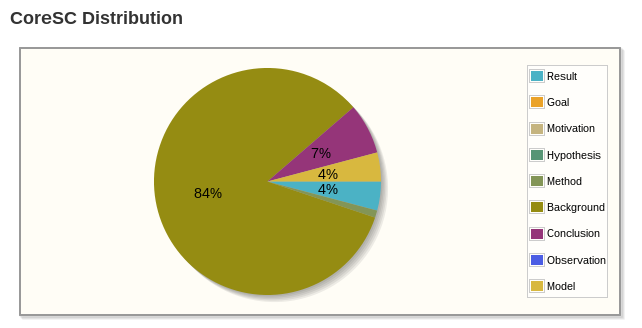
\includegraphics[width=\textwidth]{images/implementation/review_corescs.png}
\caption{CoreSC content for a sample review paper}
\end{subfigure}
\begin{subfigure}[b]{0.6\textwidth}
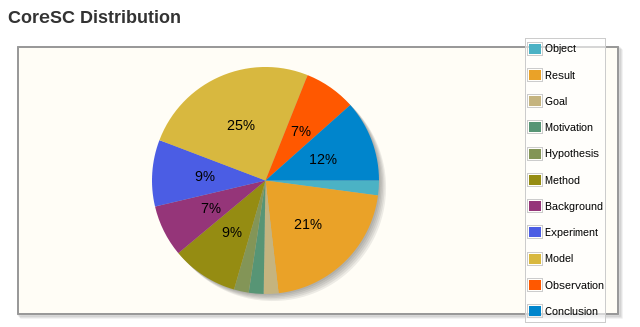
\includegraphics[width=\textwidth]{images/implementation/report_corescs.png}
\caption{CoreSC content for a sample research paper}
\end{subfigure}

\caption{Contrasting CoreSC content of Review and Research Papers}
\label{fig:coresc_pies}
\end{figure}

Figure \ref{fig:coresc_pies} shows the CoreSC content of a review paper and a
research paper randomly selected from the corpus. The review papers tend to be
made up almost entirely from Background CoreSC sentences. However, research
papers are much more evenly spread, made up of several different types of
CoreSC. This investigation suggested that there is almost certainly a discriminative
relationship between CoreSC categories and a paper's type. 

\subsubsection{ K-means clustering}

Before working with supervised learning systems, a preliminary experiment was
carried out to see whether clustering papers using the K-means algorithm could
successfully identify the paper types, thus removing the need to train and
maintain a supervised model. This was also an excellent opportunity to explore
the data and try and detect any inherent patterns within the papers.

K-means clustering uses the Euclidean distance between each data sample to
decide which cluster it is closest to and should belong to. K is the number of
clusters that are used and is decided ahead of execution. K-means clustering is
often run multiple times using a range of K values when the number of clusters
in the data is unknown. The performance of the clustering algorithm is often
evaluated using the K-means silhouette which is a measurement of how tightly
the data is clustered. A low silhouette value ($K \approx 0$) suggests loose
clustering and therefore little correlation, a high silhouette value ($K
\approx 1$) corresponds with very tight clustering and good correlation.

All of the papers were manually identified as either a ``Case Study", a
``Review Paper" or a ``Research Paper." They were then loaded into a script and
clustered using their CoreSC respective compositions. K-Means silhouettes were
used as a measure of how effective the clustering process was. This was
repeated for $ K \in [2..8] $ and the best silhouette measurement and value for
K retained. The algorithm consistently showed that K=3 was the best K value.
However, the silhouette value was consistently low. It was suggested that this
may have been because all CoreSC types were considered equally; the less
discriminative CoreSCs may have been offsetting the effect of the highly
discriminative ones.

To remedy this, all papers were again clustered, but using only three CoreSC
labels at a time: reducing the noise from the less important types. The
algorithm was run for all combinations of 3 CoreSC labels, again retaining only
the most successful combination of features and K value based upon the K
silhouette value. This returned a set of much stronger K silhouette values in
general. The algorithm also determined that the combination of ``Background",
``Motivation" and ``Method" CoreSC labels seemed to be the most
discriminative, providing a silhouette value of 0.63. 

\begin{figure}[!ht]
\centering
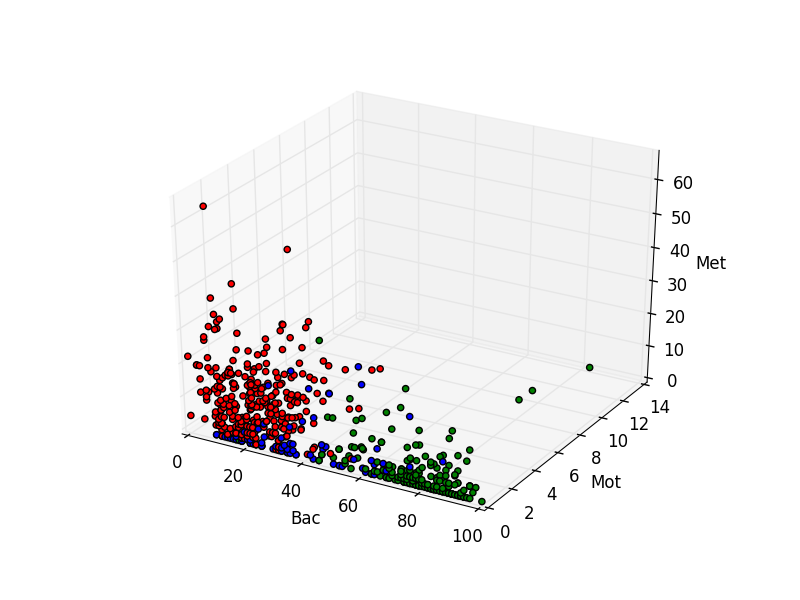
\includegraphics[width=0.8\textwidth]{implementation/cluster.png}
\caption{Paper types rendered using Bac, Met and Mot CoreSCs}
\label{fig:clusters}
\end{figure}

Figure \ref{fig:clusters} shows the papers from the corpus rendered in 3
dimensions using their Background, Method and Motivation CoreSC makeup.
Although the data does not cluster perfectly by class, these three categories
do provide fairly clear discrimination between the three types of paper. 

Clustering the papers did not seem to provide a reliable way to classify them
by type and it was decided that better results could be obtained through the
use of a supervised learning classifier instead. However, the three most
discriminative CoreSC types were chosen as features for the learner.

\subsubsection{Random Forest Learner}

To classify the papers, a Random Forest Learner was trained using a subset of
the Partridge corpus using Background, Method and Motivation CoreSC information
from the papers. The classifier was found to be highly accurate, correctly
predicting a paper's type in 87.9\% of cases. The classifier's accuracy and
evaluation are further discussed in Section \ref{sec:evaluation_learners}
below. 

The new classifier was incorporated into the paper preprocessor and triggered
after SAPIENTA annotation for each new paper. It was also called
retrospectively for papers in the Farnsworth Partridge instance that were not yet
classified.


\subsection{ Paper Processing Notifications }

Providing notifications to users when a paper has been processed was not part
of the original design for Partridge. The feature was added to the system after
being raised as a potential improvement by one of the test users. Previously,
users to added papers to the Partridge corpus did not know whether the
operation was a success unless they ran a search and the paper appeared in
their results. Adding email notifications to Partridge significantly improved
the user experience for paper uploaders. The uploader is given the option to
provide their email address when they send the paper to the Partridge server.
Once the preprocessor has converted, annotated and classified a paper, an email
is sent to the uploader informing them that the paper has been added to the
database and containing a direct link to the paper's profile page.

The system also emails users upon failure, allowing them to report the error to
the GitHub page if required and also providing closure for users who are unsure
why their paper isn't appearing in Partridge queries.



\section{ Web Backend }

The Partridge web backend was much easier to implement than the preprocessor.
The web framework Flask was used to do a lot of the hard work such as routing
requests and encoding data into browser-compatible formats.

\subsection{ Server Views }

Flask provides a model-view-controller style framework in which specific web
URLS are represented by `view' functions. The behaviour of these views changes
dependent upon data from the incoming HTTP request. Their return value is
encoded as an HTTP response and sent back to the browser that made the request.

The implementation of the server views was for the most part straight forward
with the exception of some of the responses to the interactive web elements in
the HTML markup. It was determined that the best way to communicate between
frontend and backend elements interactively was to encode responses as
JavaScript Object Notation JSON - a common notation used to describe arbitrary
data structures\cite{jsonRFC}. Despite its name, JSON encoders and decoders are
available for most common programming languages, not just JavaScript.  Flask
even has an inbuilt method called jsonify which can be used to automatically
encode arbitrary Python objects as JSON and send it back to the browser for
parsing by the frontend scripts\cite{flask2012}.

Some of the frontend scripts such as the Query Form rely upon the server to
return dynamically generated HTML markup containing data about the papers being
processed. In line with its model-view-controller architecture, flask provides
a templating module that can be used to populate pre-coded HTML templates with
data from the database on the fly. Templates for each of the views are stored
within the \emph{templates/} subdirectory within Partridge and are populated
using data retrieved from the relational database when a call to one of the
view functions is made\cite{flask2012}.

\subsection{Database Interaction \& SQLAlchemy}

Partridge makes extensive use of a relational database system for storage and
retrieval of paper data and metadata. It uses an SQL database server and
initially the schema listed in Section \ref{sec:db_layout}. Rather than using
raw SQL calls to communicate with the database, It was determined that the use
of an Object-Relation-Mapper (ORM) library such as SQLAlchemy could
significantly speed up development time. SQLAlchemy and ORM wrappers are used
to abstract database entities into language constructs. 

SQLAlchemy enables the representation of papers, authors and other entities as
Python objects. These objects can also be extended and custom methods added to
them, enabling the creation of specific entity methods such as calculating
CoreSC makeup of papers and computing first, middle and last names from a
single input string of an author's full name.

\subsection{Data version control \& Alembic}

During the development of Partridge, the structure of the SQL database used to
store the papers changed a lot due to modifications to the ORM modules as
discussed above. These structural changes meant that the production database at
\url{http://farnsworth.papro.org.uk/} and the development database were not
compatible and that updates to the code on the development server would break
the application on the production server unless the database structure was also
updated. 

To prevent this from happening, a Python utility called
Alembic\cite{alembic2013} was used for keeping the Database structure under
Version Control. Alembic is executed when Partridge's ORM models are modified
and can detect differences in database structure between the SQLAlchemy model
in Partridge's source code and the live database. It generates sets of SQL
commands that are used to synchronise the database structure with the most
recent program structure. This allowed the Farnsworth database to be updated
automatically when a new change to Partridge's data structures was made rather
than having to be purge and repopulate it.

\subsection{WSGI and Apache Integration}

Flask provides a test server that can be used for developing your web
application. However, it is written in python and is not designed to be as
stable or scalable as a full web server application such as Apache. Once
Partridge's basic web interface was complete and the application ready to be
deployed, it had to be integrated into Apache to provide stable web server
support.

By default, Apache only serves static HTML content and image/data files. It makes
use of plugins to support dynamic web pages, in languages such as PHP and
Python. A plugin called WSGI is used to allow Apache to serve Python
applications. WSGI requires that the Python program exposes an
\emph{application} object which implements a common interface in order to
communicate with Apache.

After thorough investigation, it was discovered that Flask provides a WSGI
compatible \emph{application} object. A small wrapper was written that exposes
the Flask app to WSGI and the server began to work as expected. Unfortunately,
the WSGI interface didn't allow the preprocessor daemon to be run in the
background. Therefore, a second wrapper was created that allowed the execution
of the Paper daemon as a standalone process.

\section{Web Frontend}

Partridge's web frontend required the least procedural programming and mainly
consists of HTML markup with some JavaScript. The layouts were based upon the
interface designs discussed in Section \ref{sec:web_frontend}. However, some
changes were made to the original designs during implementation to improve
usability functionality.

As discussed above, the HTML layouts were stored as templates in the
Partridge system and were evaluated and expanded using data from the SQL
server at runtime. Flask's database engine supports object oriented templates
that inherit properties from each other. This allowed the main page layout to
be designed once and reused for each specific view. 

Bootstrap, a powerful design framework was used to help build the frontend
pages and forms. Bootstrap offers a set of standard CSS and JavaScript
utilities that assist the developer in designing page layouts and provide
commonly used boilerplate code and interface elements\cite{bootstrap2013}. This
allowed the page layouts and forms used in Partridge to be implemented a lot
quicker than if they had been implemented from scratch. jQuery, a library for
manipulating HTML page layouts using JavaScript and providing utility functions
for server communication, was also used to save time in writing the interactive
aspects of frontend code. 

Whilst these libraries did not provide any assistance specific to the domains
of information retrieval or machine learning, they did help accelerate the
implementation of the frontend interfaces and provide cross-browser compatible HTML5
interfaces. Other javascript libraries providing multiple file upload
capability and browser history manipulation were incorporated into specific
user interface modules.

\subsection{Query Interface \& Results View}

After the project had been running for approximately 1 iteration, it was
decided that the query and results views were confusing and provided a
disjointed user experience for those trying to query the system. The results
view was initially designed as a separate page to the query view and
consequentially, users found it quite confusing when trying to relate the
results from the system to the query they had provided on the previous page and
it was inconvenient to have to keep changing the page when manipulating the
query. 

To improve the Partridge user experience, the query and results views were
combined into a single interactive page that used JavaScript to retrieve
results from the backend system and simply append them to the current page
using a jQuery function.

\begin{figure}[!h]
\centering
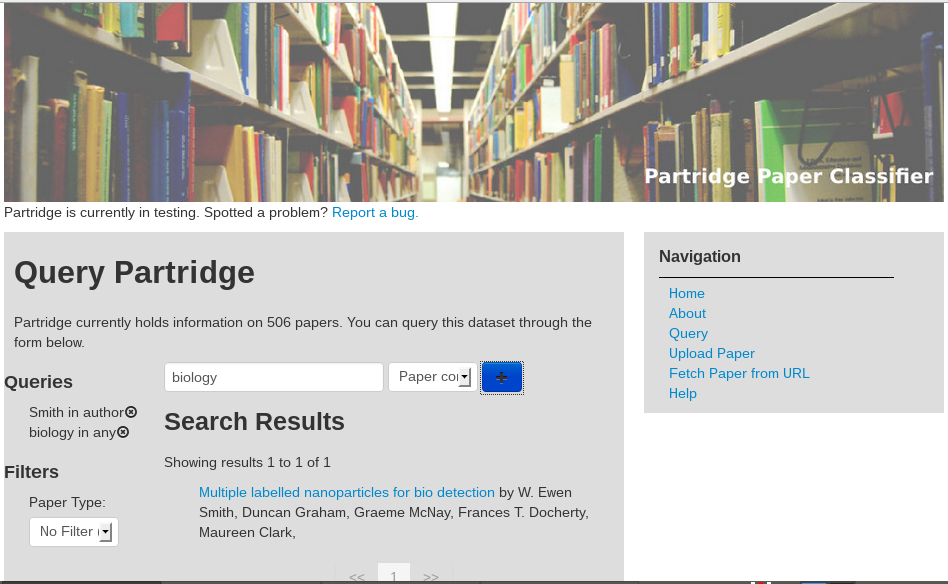
\includegraphics[width=\textwidth]{images/implementation/queryform_actual.png}
\caption{The updated query form with integrated results}
\label{fig:queryform_actual}
\end{figure}

The redesigned query form, as shown in Figure \ref{fig:queryform_actual},
allows the user to add constraints to the query one at a time using the input
field at the top of the page. These constraints are then listed on the left
hand side and can be removed by clicking on the relevant cross icon next to the
term to be removed. Filters such as paper type and topic are available in the
left toolbar and be manipulating using the relevant dropdown box. Changing any
of the filters or constraints automatically triggers the JavaScript routine to
retrieve new results from the server.

Using JavaScript to update the results and manage the query on a single page
provides a significantly better user experience. Unfortunately, it does
interfere with how browser handle a user's history, breaking the Back and
Forward buttons in all browsers and preventing users from linking to their
query results and posting them to friends or colleagues.

The jQuery BBQ (jqBBQ) library was used to restore this functionality
\cite{jqbbq2013}. The library allows the scripted manipulation of the URI
fragment, a string that forms part of a page's URI but does not change the HTTP
request made to the server\cite{urifragment2013}. The fragment can be used to
serialise the the state of the user interface, allowing users to share links to
search results and restoring browser history functionality. A javascript
function was set up to fire when the interface was fully loaded and examine the
URL fragment, converting key, value pairs into search constraints. A
serialisation function was also set up to trigger whenever search constraints
and filters were added and removed from the query and update the fragment
string accordingly.

\subsection{ Paper Upload Interface }

The paper upload interface was initially designed to allow authors of papers to
submit their work to be analysed by Partridge and display the upload progress
in the form of a horizontal progress bar on the page. Normally, web browsers
only allow the selection of one file at a time for upload and makes an HTTP
request with the file data, without telling the user how long it might take or
providing any information on the upload progress. To implement multiple file
uploads and a progress bar, a significant amount of JavaScript code is
required. 

jQuery HTML5 Upload was used to speed up implementing this feature. This
library provides an interface for uploading files asynchronously within the
user's web browser and triggering a callback method when progress is made
during an upload and when a file ha finished uploading. This allowed the
implementation of a progress bar and text readout of the upload progress
without forcing the browser to refresh the page.

After reviewing the design of the page, a new checkbox was added to the upload
form that forces the user to verify that they have permission to upload the
paper in an attempt to prevent problems with copyright and ownership issues.
The users are also linked to \url{http://www.sherpa.ac.uk/romeo/}, a service
that can be used to identify the copyright policy of paper authors and
journals and whether specific papers can be used by Partridge. 

\subsection{ Bookmarklet }

One of the most important user suggestions for improving the usability of
Partridge and facilitating the rapid expansion of the paper corpus was the
Paper Upload Bookmarklet. The bookmarklet was not in the initial system design
and was added as an extra feature towards the end of the project. It allows
users browsing sites such as PubMed Central and PlosOne to add papers that
interest them to Partridge without having to download the paper from the
journal and upload it to the Partridge server manually. 

The system is implemented as a standard web page wrapped inside a JavaScript
module that can be added as a bookmark to a user's web browser. When the user
finds a paper that they wish to add to Partridge on one of the compatible
journal sites, they click the bookmark, loading an embedded frame in their
current browser window and automatically uploading the paper that the user is
looking at to Partridge's server. 

The bookmarklet trivialises the act of adding new papers to Partridge and this
should help to encourage users to help grow Partridge's paper corpus as quickly
as possible. It should also remove complications surrouding the rights of authors and
publishers of papers since it is only compatible with sites that publish open
access articles and cannot be used to add papers to Partridge that may be
copyright protected.

\section{Summary}

Partridge's implementation took place over a period of many weeks, with
incremental improvements, often stemming from user suggestions, being
incorporated throughout. There were several deviations from the original
project designs. Nonetheless, most of the designs were appropriate and provided
an excellent starting point for implementation of the project.

The effective and appropriate use of libraries within Partridge helped in
speeding up the development of the project using well tested and maintained
code from other developers. This required a different skillset which could be
considered equally or more important than just writing new code
\emph{vis-à-vis} a holistic understanding of the nature of the project and the
relationships of the core modules. Working with libraries requires
comprehensive conceptualisation of the task at hand whereas programming
requires focus on a specific subset of the component's behaviour and attaining
expected outputs for given inputs to the routine under construction.
